\documentclass[9pt,sigconf]{acmart}
\usepackage[utf8x]{inputenc}
\usepackage{ucs}
\usepackage{amsmath}
\usepackage{amsfonts}
\usepackage{amssymb}
\usepackage{graphicx}
\usepackage{booktabs}
\usepackage{listings}
\usepackage{courier}
\usepackage{color}
\usepackage{stfloats}

\settopmatter{printacmref=false}
\renewcommand\footnotetextcopyrightpermission[1]{}

\title{Local Common Subexpression Elimination}
\subtitle{Report of Assignment 2}

\author{Chih-Yung Liang}
\affiliation{
	\department{Graduate Institute of Networking and Multimedia}
	\institution{National Taiwan University}
}
\email{r05944012@csie.ntu.edu.tw}

\author{Shih-Kai Lin}
\affiliation{
	\department{Dept. of Computer Science \& Information Engineering}
	\institution{National Taiwan University}
}
\email{r05922043@csie.ntu.edu.tw}

\lstset{
	basicstyle=\ttfamily,
	language=bash,
	morekeywords={mkdir, cmake, make, opt},
	deletekeywords={test},
	commentstyle=\color[rgb]{0,0.6,0}\textit,
	keywordstyle=\color{magenta},
}

\begin{document}
	\maketitle
	
	\begin{figure*}[bp]
		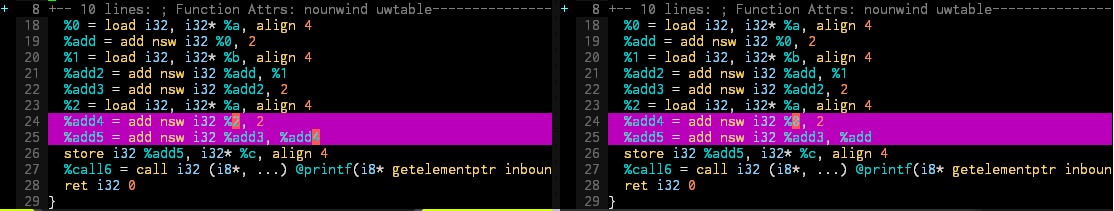
\includegraphics[width=\textwidth]{demo}
		\caption{Test result for the test \textit{eli-adds1}}
		\label{fig:test-result}
	\end{figure*}
	
	\section{Methodology}
	To reuse common subexpressions in a local region, the transformation is implemented as a \textit{BasicBlockPass} that iterates each basic block of given code region. A map data structure, named \textit{ExprHash}, mapping expressions formed with operands and operation kind to already existed instructions is used to record reusable expressions. The key-value pair \textit{ExprHash} stores is:
	$$
	\begin{aligned}
	Key &: \text{OpCode (as \textit{unsigned}) and 5 Operands (as \textit{Value *})}\\
	Value &: \text{Exist instr. that evaluates the expression (as \textit{Value *})}
	\end{aligned}
	$$
	It is noticeable that for expressions not requiring as many as 5 operands, the extra unused operand fields of the key of \textit{ExprHash} are marked empty with \textit{nullptr}.
	
	The procedure of the transformation is to iterate each reusable instruction in the basic block under processing and store the expression the instruction evaluates in \textit{ExprHash}, where reusable ones are instructions of types defined in Table~\ref{tab:reusable-types}. For expressions already in \textit{ExprHash}, instead of re-insert into \textit{ExprHash}, use exist evaluator instructions to replace all uses of duplicated expression evaluators. However, store instructions between load instructions with common expression can modify the data to load and invalidates exist evaluated load results.
	
	\subsection{Memory Modification Handling}
	When the basic block iteration reaches a memory writing instruction, the transformer has to check if the written address aliases any address read by memory reading instructions in \textit{ExprHash}. It has to be conservative, so only memory reading instructions, which must be load instructions, that are sure not to alias the memory writing instruction, which must be a store instruction, are kept in \textit{ExprHash}; otherwise, they are removed from the map. The alias analysis result is taken from \textit{BasicAliasAnalysis} provided by LLVM itself, which basically distinguishes different globals, stack allocations, and heap allocations. Indexes into arrays with statically differing subscripts are also reported as \textit{NoAlias} by the alias analysis result.
	
	\section{Building \& Testing}
	\subsection{Building the Program with CMake}
	\begin{lstlisting}
$ # Building
$ mkdir build && cd build
$ cmake .. && make
$ # Usage
$ opt -load Transform/MyPass.so -my-cse ...
	\end{lstlisting}
	
	\subsection{Testing CSE with CTest}
	The test script automatically compiles C sources into LLVM IR with \textit{Clang}, performs the transformation with \textit{Opt}, and compares the difference made by the transformation using \textit{Vimdiff}. The usage of the script is:
	\begin{lstlisting}
$ make CSE-test-<test name>
$ # For example:
$ make CSE-test-eli-adds1
	\end{lstlisting}
	Table~\ref{tab:tests} lists available tests for the transformation, where the source for each test is placed under \texttt{Tests/CSE}. Figure~\ref{fig:test-result} illustrates the test result of \textit{eli-adds1}.
	
	\begin{table}[t]
		\caption{Types of Reusable Instruction}
		\label{tab:reusable-types}
		\begin{tabular}{|c|c|c|}
			\hline
			BinaryOperator & CmpInst & ExtractElementInst \\
			\hline
			GetElementPtrInst & InsertValueInst & InsertElementInst \\
			\hline
			PHINode & SelectInst & ShuffleVectorInst \\
			\hline
			CastInst & ExtractValueInst & LoadInst \\
			\hline
		\end{tabular}
	\end{table}

	\begin{table}
		\caption{Available Tests}
		\label{tab:tests}
		\begin{tabular}{|c|c|c|c|c|}
			\hline
			noeffect1 & noeffect2 & noeffect3 & eli-loads1 & eli-loads2 \\
			\hline
			eli-loads3 & eli-adds1 & eli-adds2 & eli-adds3 & eli-ptr1 \\
			\hline
			eli-ptr2 & eli-ptr3 & eli-ptr4 & & \\
			\hline
		\end{tabular}
	\end{table}
\end{document}